\section{Theorie}
\label{sec:Theorie}
Alle Bilder und Informationen wurden aus dem Dokument \cite{v406} entnommen.\\
\subsection{Baiscs zur Beugung}
Es wird von Beugung gesprochen, sobald die geometrische Optik die Lichtausbreitung nicht mehr erklären kann. 
Dies tritt auf, wenn das Licht durch Öffnungen oder auf undurchlässige Öffnungen trifft. 
Dazu müssen die Abmessungen der Aperaturen kleiner als der Strahlendurchmesser sein.
Die Beugung wird hinreichend beschrieben, wenn das Licht als Wellenphänomen betrachtet wird.
\subsection{Huygenssches Prinzip}
Um die beobachteten Ergebnisse erklären zu können, wird zunächst das Huygenssche Prinzip betrachtet.
Dieses Prinzip besagt, dass jeder Punkt einer Elementarwellenfront an einem Hindernis ein Fundament für eine Kugelwelle ist.
Diese neu entstandenen Kugelwellen interferieren und bilden eine neue Wellenfront, welche der Einhüllenden der Elementarwellen gleicht.
Somit können die neuen Wellen in den geometrischen Schattenraum eintreten.
\subsection{Fraunhofersche Beugung}
\begin{figure}
    \centering
    \caption{Fraunhofer Beugung}
    \label{fig:Fraunhofer}
    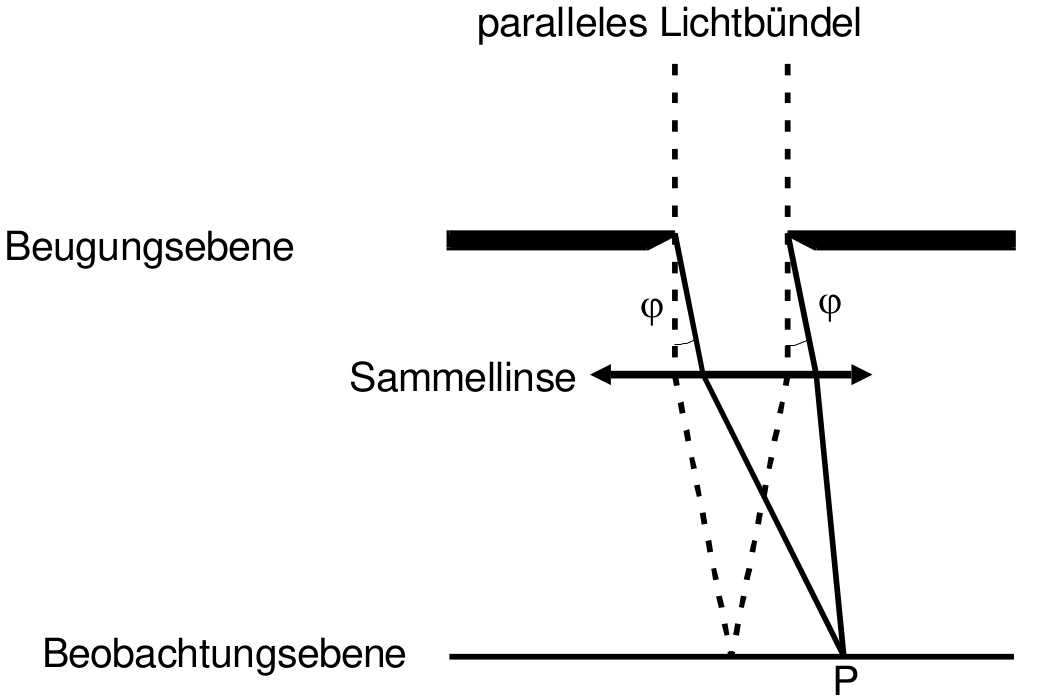
\includegraphics[width = 0.5 \textwidth]{pics/Frauenhofer.PNG}
\end{figure}
Um die Beugung beschreiben zu können, wir die Frauenhofersche Beugung verwendet.
Dazu wird angenommen, dass die Elementarwellen von einer in unendlicher Ferne stehender parallel ausgesendet werden.
Daraus folgt, dass der Beugungswinkel $\varphi $ von den Strahlen, die in einem Punkt P (\ref{fig:Fraunhofer}) interferieren,
der selbe ist. 
Somit ist es im Vergleich zu anderen Näherungen einfacher, dass Problem mathematisch zu verfassen.
Hierbei werden nur Spalte betrachtet, dessen Länge sehr groß gegen die Breite ist, so dass nur eine eindimensionale Betrachtung von Nöten ist.
\subsection{Amplituden- und Intensitätsfunktion}
Zunächst wird eine Welle mit der Feldstärtke 
\begin{equation}
    A(z, t) = A_0 \, \symup{e}^{\symup{i} \left (\omega t - \frac{2\symup{\pi}}{\lambda} \right )}
\end{equation}
betrachtet.